\chapter{Experimental study}
\startcontents[chapters]

\section{Methodology}
We decided to test speakers' preferences for syntactic and semantic agreement in two online experiments: one using one type of lexical hybrids, profession nouns referring to women, the other using split hybrids, depreciative forms which have a form of non-masculine nouns, but refer to men. In the experiments we tested predicative verb agreement and relative pronoun agreement.

I submitted the design of the experiments and the materials to the Paris Graduate School of Linguistics Ethics Committee and got their approval in May 2026. The following subsections describe the experiments in more detail.

\subsection{Procedure}
We conducted two acceptability judgement experiments: one using stimuli with profession nouns and the other with depreciative forms. Both experiments had the same design, which was 3x2 within-subject. The independent variables were the agreement options (semantic or syntactic) and type of agreement with ordering of target and controller: predicate with target first (prenominal), predicate with controller first (postnominal) and relative pronoun (always with controller first, since it is impossible to place the relative pronoun before its antecedent). The dependent variable was the rating of acceptability of given sentences.

The experiment was conducted in Polish. It was recommended to participants to complete the experiment using a computer or tablet, to make sure the instructions and stimuli were displayed correctly. On the first page participants were told their task was to judge whether the displayed sentences sounded naturally or not. They were also informed that participation in the study was voluntary and they could withdraw at any time. To proceed to the study they had to tick a box to confirm they consent. Next, they saw the instructions page, which had the following information.

{\slshape
  Your task will be to judge how naturally the displayed sentences sound. If you aren't sure what this means, consider whether you could hear or say the given sentence. You will judge the sentences on a 5-point scale, from ``completely unnatural'' to ``completely natural''. You will see a control question after each sentence.

  Before we proceed to the study, you will see 3 practice questions that will allow you to familiarize yourself with the task. After the practice session you will proceed to the study, which consists of 60 questions. During the study you cannot go back to the previous questions and there is no time limit to answer the questions, but answer intuitively, without thinking too much.
}

Out of 60 trials, 24 were with experimental items. They were arranged using the Latin square design -- in 6 lists, so that each item appears on a list once and each list has 4 items per condition. Each participant was assigned a list randomly and the order of items was randomized each time. Each trial was followed by a simple comprehension question, to ensure that participants are paying attention to the experiment.

In the experiment on profession nouns the instruction in each trial was ``Read the sentences below and judge how naturally the \textbf{\textsl{second}} one of them sounds'', for the experiment on depreciative forms it was ``Read the sentence below and judge how naturally it sounds''. As was said in the instructions for participants, judgements were given on a 5-point scale. Such a scale is familiar for Polish speakers, because it is similar to the grading scale in Polish schools (1-6 with 6 being the best) and in Polish universities (2-5 with 5 being the best). The scale was labelled only on the ends with \mean{całkowicie nienaturalne}{completely unnatural} and \mean{całowicie naturalne}{completely natural}.

After participants gave judgements on 60 sentences, there was a short demographic survey asking about their age, gender, first language(s) and the country or countries where they were raised. All of the response fields for those questions allowed for any kind of text answer to be typed. The duration of the whole experiment was 15-20 minutes.

\subsection{Materials}
Experimental items were constructed so that the agreement controller was either in the first or the final position in the sentence, the agreement target was immediately adjacent to the controller and there were no other words in the sentence that agreed with the controller in gender. To make sure that the last constraint was not violated, all of the sentences with relative pronoun agreement had to be in present tense (because predicates in present tense do not agree with the subject in gender), while the sentences in other conditions were in past tense. The following subsections describe how the nouns for the experimental items were selected.

\subsubsection{Experimental items with depreciative forms}
Depreciative forms appear in the paradigms of \textsc{m1} nouns and morphologically they resemble nouns of genders other than \textsc{m1}. In Corbett's approach then, when using those nouns in a sentence we have a syntactic reason to use non-\textsc{m1} agreement and a semantic reason to use \textsc{m1} agreement. To make sure that semantic reason is clearly pointing to \textsc{m1}, the nouns selected for this experiment had to be commonly perceived as masculine. To ensure that, the selection process relied on a norming study conducted by \cite{misersky_norms_2014}, where they collected information about gender stereotypicality for role nouns in multiple Eurpean languages.

There were 22 nouns that fulfilled the following criteria:
\begin{itemize}
  \item Perceived to be at least 60\% masculine according to the norming study.
  \item Appear at least a 1000 times in the balanced version of the National Corpus of Polish.
  \item Depreciative form is not syncretic with the non-depreciative.
  \item Does not have disturbing, violent connotations (e.g. \textsl{rapist}, \textsl{murderer})
  \item Depreciative form is not syncretic with a different noun (e.g. noun \mean{technik}{technician} is \textsl{techniki} in depreciative, which has the same shape as the word for `techniques' and could lead to confusion)
  \item Is not a nominalized adjective (for which depreciative forms are syncretic with the feminine versions of these nouns)
\end{itemize}
Additionally, there were two nouns that did not occur in the norming study: \mean{proboszcz}{parish priest} and \mean{chłopak}{boy}. The former fulfills all of the criteria above, besides being perceived as at least 60\% masculine in the norming study, since it is not included there. However, it can be included in the experiment because it is a noun commonly used in Polish and, as a subtype of a priest, it counts as being perceived as masculine.

As \cite{skowronska_konstrukcje_2011} reports, the latter of the two additional nouns is problematic for Polish speakers. In a section dedicated specifically to the lexeme `chłopak' she reports that some Polish speakers are taught that the non-depreciative form of the noun is incorrect. Because of this, hybrid agreement is very commonly used with this particular noun. The author also looked through the National Corpus of Polish to see a few examples of the noun with attributive and predicate agreement and she finds that predicates with this noun are mostly seen with semantic agreement, while attributes occur almost exclusively with syntactic agreement. This is in line with Corbett's predictions and the current study can test whether this tendency extends to the further points of the Agreement Hierarchy.

All of the nouns chosen for this experiment can be found in the Appendix (Table ?). In (\ref{ex:depr-item}) there is an example of an experimental item with one of the nouns in depreciative form. 

\begin{exe}
  \ex\label{ex:depr-item} Example of an item in the experiment with depreciative forms in all conditions and with its comprehension question.
  \begin{xlist}
    \ex f/m1, prenominal
    \gll Na nagrania do Ameryki Południowej poleci-ały/poleci-eli reżyser-y.\\
    for shooting in America South flew\textsc{-pst.3pl.nm1}/flew\textsc{-pst.3pl.m1} directors\textsc{-pl.nom.depr}\\
    \glt ``The directors flew to South America for shooting.''\\
    
    \ex f/m1, postnominal
    \gll Reżysery poleci-ały/poleci-eli na nagrania do Ameryki Południowej.\\
    directors\textsc{-pl.nom.depr} flew\textsc{-pst.3pl.nm1}/flew\textsc{-pst.3pl.m1} for shooting to America South\\
    \glt ``The directors flew to South America for shooting.''\\
    
    \ex f/m1, relative pronoun
    \gll Reżysery, któr-e/któr-zy lecą na nagrania do Ameryki Południowej, nie odpowiadają teraz na maile.\\
    directors\textsc{-pl.nom.depr} who\textsc{-nm1.pl.nom}/who\textsc{-m1.pl.nom} fly for shooting to America South \textsc{NEG} responding now to emails\\
    \glt ``Directors, who are flying to South America to shoot, are not responding to emails right now.''\\

    \ex comprehension question\\
    Czy w zdaniu wspomniano o Azji?\\
    \textsl{Did the sentence mention Asia?}
  \end{xlist}
\end{exe}

\subsubsection{Experimental items with profession nouns}
The process of selecting nouns for this experiment was similar to that for the corpus study. The study by \cite{szpyra-kozlowska_premiera_2019} was used to find masculine nouns, for which it is difficult to use a feminine version. Nouns were arranged from the most times participants of the study refused to give a feminine version of the noun, to the least. This formed a ranking, from which the following nouns were excluded:
\begin{itemize}
\item \mean{ksiądz}{priest}, \mean{pastor}{pastor} and \mean{proboszcz}{parish priest}, because in Poland the population of female priests is almost nonexistent
\item offensive words (e.g. \mean{dureń}{fool})
\item words with less than a 1000 occurrences in the balanced version of the National Corpus of Polish (with literature excluded to make sure the words are used in everyday language)
\end{itemize}

Here each experimental item also required a sentence of context preceding the target sentence. The nouns used in this experiments are masculine and can refer to both men and women, so context is needed for participants to know that in this situation the noun refers to a woman. All of the items for this experiment can be found in the Appendix (Table ?) and an example of an item can be found in (\ref{ex:prof-item}).

\begin{exe}
  \ex\label{ex:prof-item} Example of an item in the experiment with profession nouns in all conditions, with its context and the comprehension question.
  \begin{xlist}
    \ex context\\
    W tym tygodniu odwiedzają nas mamy uczniów z naszej klasy, żeby opowiedzieć o swojej pracy.\\
    \textsl{Moms of kids from our class are visiting us at school this week to talk about their careers.}
    
    \ex f/m1, prenominal
    \gll We wtorek przysz-ła/przysz-edł architekt-Ø.\\
    on Tuesday came\textsc{-pst.3sg.f}/came\textsc{-pst.3sg.m} architect\textsc{(m1)-sg.nom}\\
    \glt ``The architect came on Tuesday.''\\
    
    \ex f/m1, postnominal
    \gll Architekt-Ø przysz-ła/przysz-edł we wtorek.\\
    architect\textsc{(m1)-sg.nom} came\textsc{-pst.3sg.f}/came\textsc{-pst.3sg.m} on Tuesday\\
    \glt ``The architect came on Tuesday.''\\
    
    \ex f/m1, relative pronoun
    \gll Architekt-Ø, któr-a/któr-y przyjdzie we wtorek, należy do Rady Rodziców.\\
    architect\textsc{(m1)-sg.nom} who\textsc{-f.sg.nom}/who\textsc{-m.sg.nom} will.come on Tuesday belongs to council of.parents\\
    \glt ``The architect who will come on Tuesday is a member of the Parents' Council.''\\

    \ex comprehension question\\
    Czy dzień tygodnia, który był wspomniany w zdaniu, to czwartek?\\
    \textsl{Was Thursday the day of the week mentioned in the sentence?}
  \end{xlist}
\end{exe}

\subsubsection{Other items}
Both experiments also had 12 control items, half correct, to establish a threshold of acceptable and unacceptable sentences and test participants' sensitivity to gender agreement. The incorrect sentences contained an attraction error with the subject, the correct ones were the same but without the error. Half of the controls had human subjects and half had non-human, this was distributed evenly within the conditions. In the profession nouns experiment these items were preceded by a sentence of context, so that the experimental item would not be too easy to distinguish. An example of a control item can be found in (\ref{ex:control-item}).

\begin{exe}
  \ex\label{ex:control-item} Example of a control item in both conditions and the context sentence.
  \begin{xlist}
    \ex context\\
    Nie wszystkie dzieci chciałyby mieć wieczne wakacje.\\
    \textsl{Not all kids want to be on holidays forever.}

    \ex correct/incorrect
    \gll Syn-Ø sąsiad-ki jest szczęśliw-y/*szczęśliw-a że idzie do szkoły.\\
    son\textsc{(m1)-sg.nom} neighbor\textsc{(f)-sg.gen} be\textsc{(prs.3sg)} happy\textsc{-m.sg.nom}/*happy\textsc{-f.sg.nom} that goes to school\\
    \glt ``The son of the neighbor is happy to go to school.''\\
  \end{xlist}
\end{exe}

To make sure the main focus of the study is not too obvious to participants, there were also 24 filler items. As with control items there was a context sentence preceding the fillers in the profession noun experiment. An example can be found in (\ref{ex:filler-item}).

\begin{exe}
  \ex\label{ex:filler-item} Example of a filler item with its context.
  \begin{xlist}
    \ex context\\
    Szukam zeszytu w którym babcia zapisywała hasła.\\
    \textsl{I'm looking for the notebook where grandma wrote down her passcodes.}

    \ex 
    \gll Znalazłem na strychu sejf i nie wiem jak go otworzyć.\\
    found on attic strongbox and \textsc{neg} know how it open\\
    \glt ``I found a strongbox in the attic and I don't know how to open it.''\\
  \end{xlist}
\end{exe}

\subsection{Participants}
Participants for both studies were recruited using Prolific. The target population on the platform was filtered to only include people who currently live in Poland, have Polish nationality and speak Polish as their first language. There were in total 60 participants (44 men and 16 women), their age ranged from 18 to 55. They were paid 3.20 GBP (3.7 EUR) for participation. This is 15.69 PLN for 20 minutes which corresponds to 47.07 PLN hourly, so around 150\% of minimum hourly wage in Poland as of 2026. 

\subsection{Hypotheses}
Based on my corpus study, one hypothesis is that syntactic agreement is preferred over semantic for depreciative forms (possibly for profession nouns too), so items with semantic agreement should have an overall lower acceptability rating than the items with syntactic agreement. The semantic agreement should, however, be rated higher than the ungrammatical control sentences.

Additionally, according to the constraint of Corbett's Agreement Hierarchy, the acceptability of semantic agreement should increase as we go rightwards along the hierarchy. Here this means that semantic predicate agreement has a lower average acceptability rating than semantic relative pronoun agreement. Another hypothesis concerns the Hierarchy of Agreement Sources, based on which semantic agreement with split hybrids is less acceptable than with lexical hybrids. For this study the split hybrids are depreciative forms and lexical hybrids are profession nouns, therefore semantic agreement in the the profession nouns experiment should have an overall higher acceptability than semantic agreement in the depreciatives experiment. Finally, according to Corbett the target of agreement preceding the controller decreases the likelihood of semantic agreement, so in the experiments the prenominal condition should have a lower acceptability than the postnomial condition. In terms of statistical modeling, this means there should be an interaction between agreement and ordering, so that semantic agreement in the prenominal condition is rated lower than in the postnominal condition.

\section{Results}
There were 30 participants invited to participate in each study. Experiment 1 (with profession nouns) had 19 men and 11 women, Experiment 2 (with depreciative forms) had 25 men and 5 women. Participants were aged 18 to 55. Out of them, one responded that he was raised in England and Poland, three reported to speak both Polish and English as their first languages. These participants were excluded from analysis, to make sure the judgements were those of monolingual Polish speakers. All participants responded correctly to comprehension questions over 80\% of the time and all of them rated the ungrammatical control questions below the grammatical ones, therefore none of them were excluded based on those criteria. There were, however, two participants in Experiment 2 that rated all experimental items as completely unacceptable. This was presumably because the depreciative forms are highly colloquial and some speakers find those forms to be ungrammatical. Those judgements were therefore not informative for the purposes of this study and responses from those two speakers were excluded. Table \ref{tab:exp-participants} shows the numbers of participants included in the analysis grouped by gender, age group and experiment.

\begin{table}[h]
  \centering
  \begin{tblr}{
    vlines,hlines,
    cell{1}{2} = {c=3}{c},
    cell{1}{5} = {c=3}{c},
    cell{1}{1} = {r=2}{c}
    }
    & Experiment 1 & & & Experiment 2 & & \\
    & 18-30 & 31-50 & 51+ & 18-30 & 31-50 & 51+ \\
    Women &   6 &   3 &   1 &   2 &   2 & 0 \\ 
    Men &  15 &   4 & 0 & 15 &   5 &   1\\
  \end{tblr}
  \caption{Numbers of participants in each age and gender group in each experiment.}
  \label{tab:exp-participants}
\end{table}

\begin{figure}[h]
  \centering
  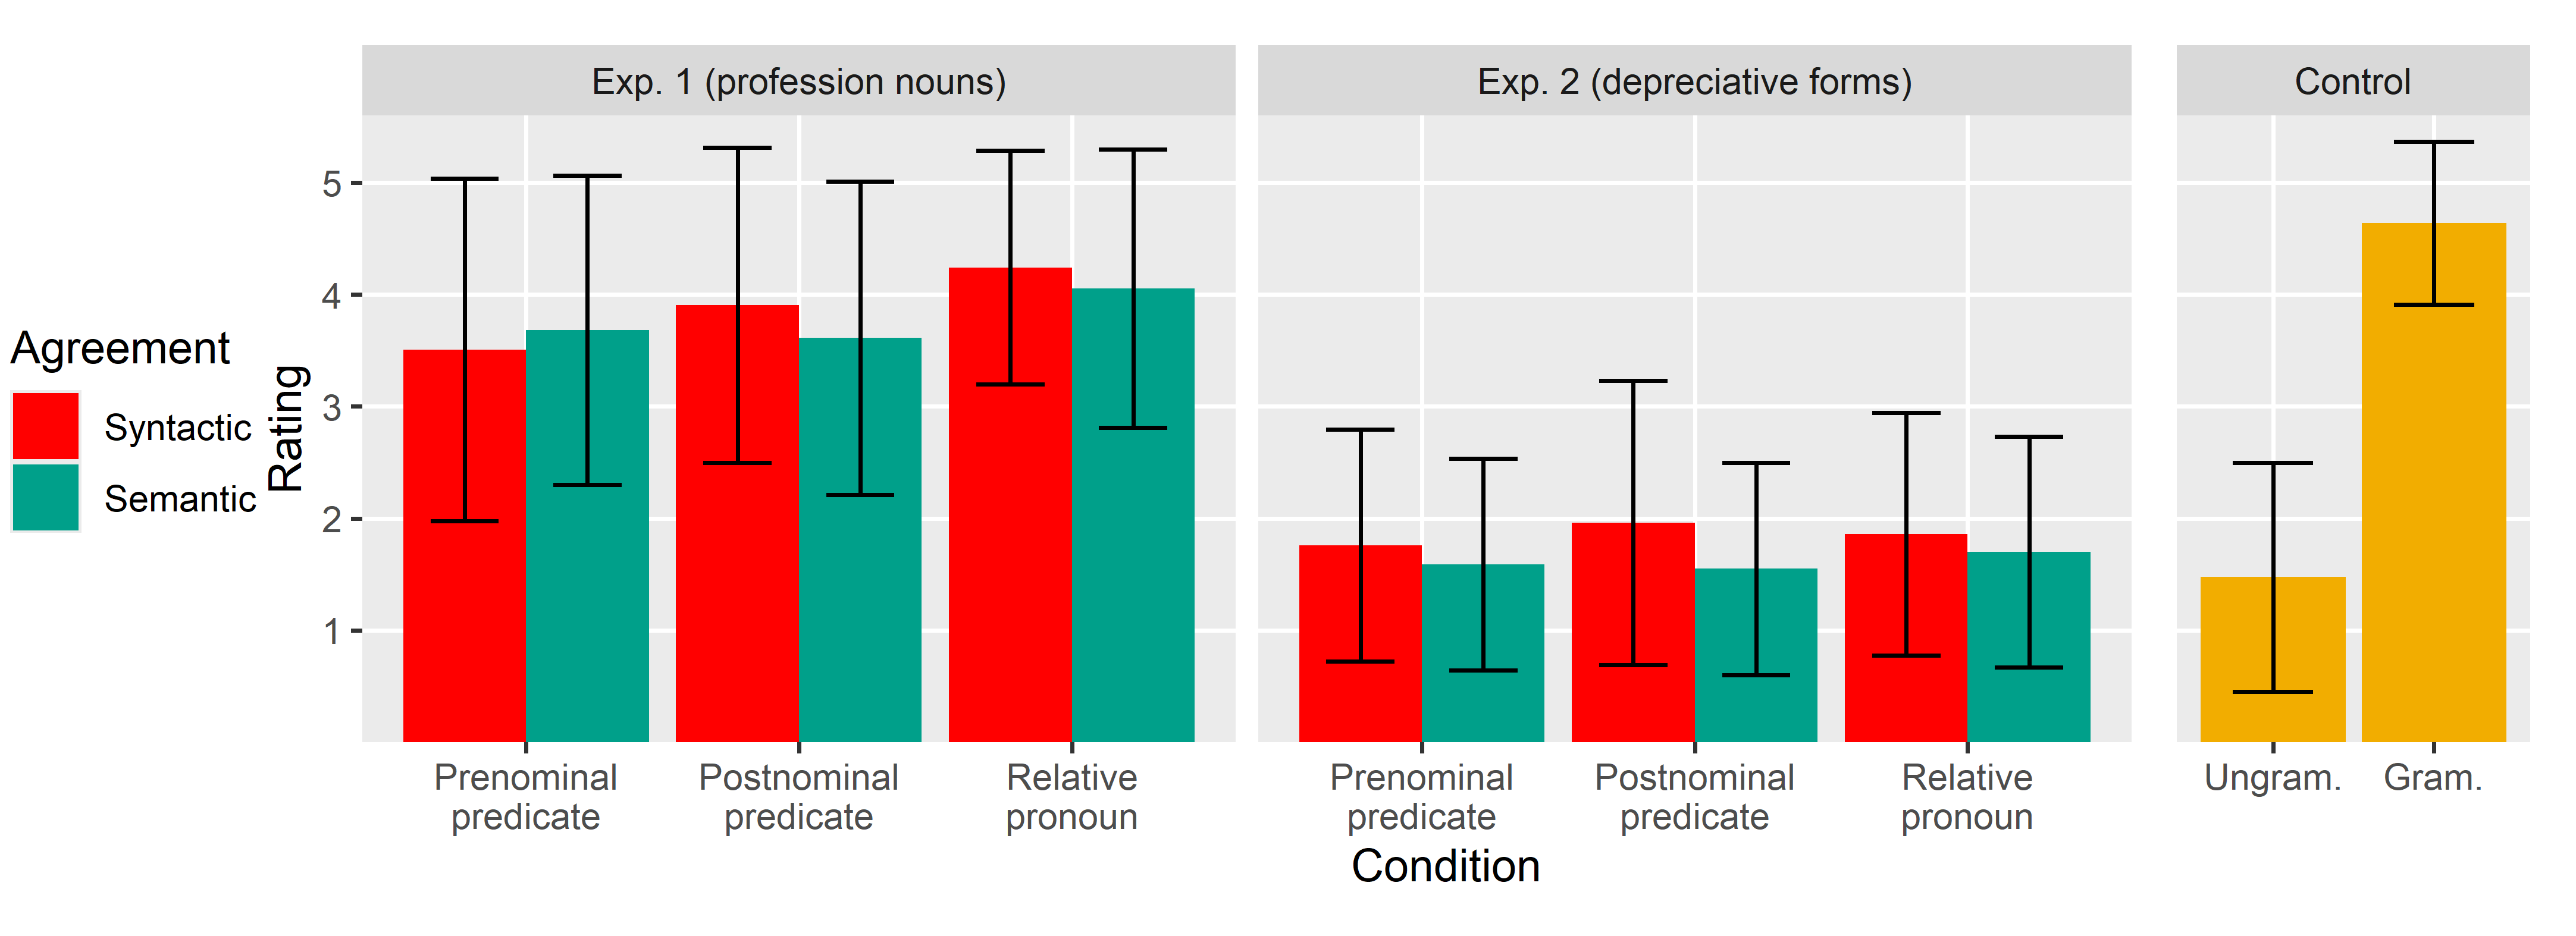
\includegraphics[scale=.7]{./images/expmainplot.png}
  \caption{Average acceptability judgements for experimental and control conditions in both experiments.}
  \label{fig:exp-main}
\end{figure}

The results of both experiments with the control conditions for comparison can be found in Figure \ref{fig:exp-main}. Overall, semantic agreement was rated as high or higher than syntactic agreement. We can see that none of the experimental conditions were on average rated lower than ungrammatical controls, although the items with depreciative forms in Experiment 2 come close to that. We hypothesised that semantic agreement will be less acceptable with depreciative forms (which are split hybrids) than with profession nouns (which are lexical hybrids). While there is a difference between the two types of nouns used, it does not depend on agreement -- items with depreciative forms received overall lower ratings than items with profession nouns. There are also differences between ratings of semantic and syntactic agreement in each condition. We can have a closer look at those differences in Figure \ref{fig:exp-diffs}. Here we can clearly see that semantic agreement was rated higher than syntactic agreement in all conditions except for prenominal predicates with profession nouns.

\begin{figure}[h]
  \centering
  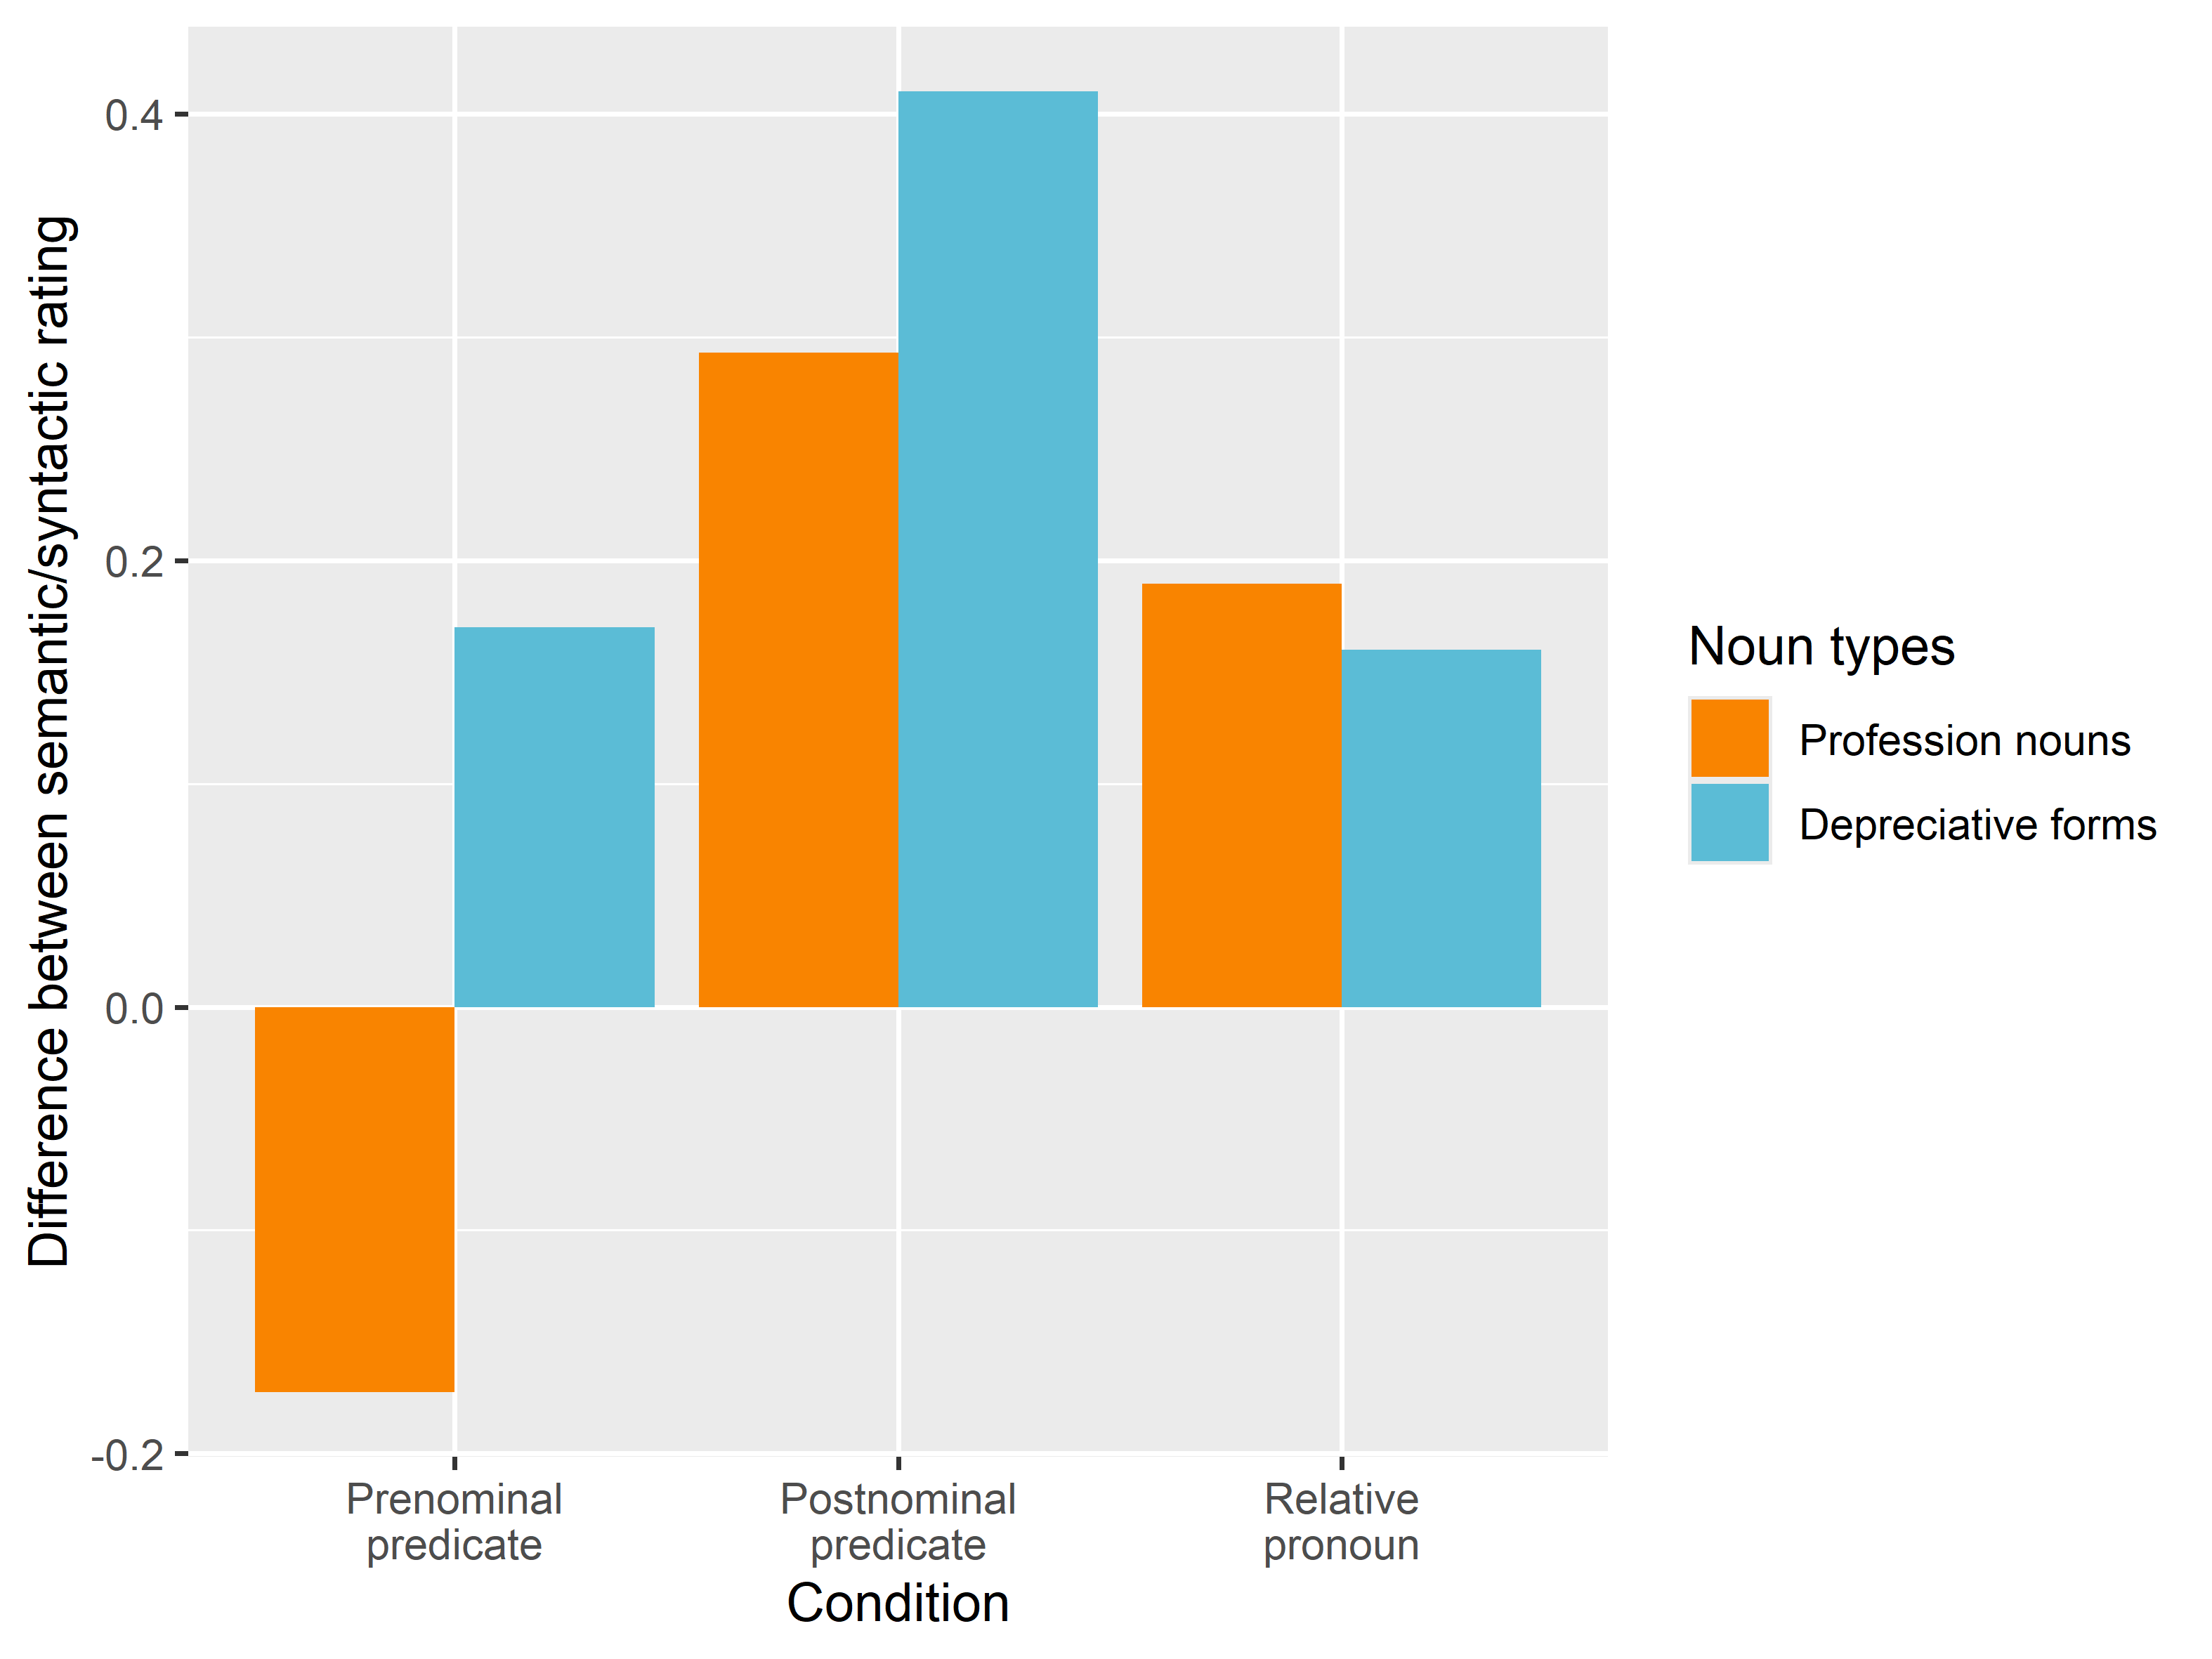
\includegraphics[scale=.8]{./images/expdiffsplot.png}
  \caption{Differences between average ratings of semantic and syntactic agreement in both experiments and in all conditions. Positive values mean that semantic agreement was rated higher than syntactic.}
  \label{fig:exp-diffs}
\end{figure}

Based on the simple constraint of the Agreement Hierarchy \citep{corbett_agreement_2023} there should be a monotonic change of preference from one value to another. This means that, for instance, syntactic agreement is clearly preferred for attributes, predicate agreement can have both syntactic and semantic agreement and relative pronouns mostly have semantic agreement. In this situation the difference in acceptability of semantic and syntactic agreement for attributes is larger, for predicates smaller, and for relative pronouns larger again (only in a different direction than for attributes). Additionally, there is the full constraint which states that as we go from attributes towards pronouns, that monotonic change of preference should mean an increase in acceptability of semantic agreement (exactly as in the described example).

Here, we can not actually test the monotonicity of change in preference, since only two possible targets from the Agreement Hierarchy were included in the study, but we can look if the differences between preferences for semantic agreement change as expected. Looking at differences for postnominal predicates (which are more canonical than prenominal) and relative pronouns in Figure \ref{fig:exp-diffs} we can see that in both experiments semantic agreement is preferred, because the differences are positive. However, the differences are larger for postnominal predicates than for relative pronouns, which can give us suggestions about the monotonicity of change of preference for one agreement option or the other.

We analyzed the results from both experiments with a mixed-effects ordinal regression model using the clmm() function from the ordinal R package \citep{ordinal}. In this model the fixed effects were the noun type (profession noun or depreciative form), agreement (semantic or syntactic), order of target and controller and the type of target (predicate or relative pronoun). The model also included interactions between the noun type and agreement and all other variables. The random effects were for participants, items, order in which items were presented, age and group from the latin square design. The full list of coefficients from this model can be found in Appendix (Table \ref{tab:coef-exp-both}).

The only significant effect in this model was the effect of noun: items with profession nouns had significantly higher ratings than items with depreciative forms (p<0.001). The following subsections will describe the analyses for the two experiments separately.

\subsection{Experiment 1}
Experiment 1 used stimuli with profession nouns. Table \ref{tab:exp-prof-summary} shows a summary of the results in this experiment.

% latex table generated in R 4.5.2 by xtable 1.8-8 package
% Sat May 30 20:32:22 2026
\begin{table}[h]
  \centering
  \begin{tblr}{
    hlines,vlines,
    cell{1}{1} = {r=2}{c},
    cell{1}{2} = {c=2}{c},
    cell{1}{4} = {c=2}{c},
    cell{1}{6} = {c=2}{c}
    }
    Agreement & Prenominal predicate & & Postnominal predicate & & Relative pronoun & \\
              & Mean & SD & Mean & SD & Mean & SD \\ 
    Semantic & 3.51 & 1.53 & 3.91 & 1.41 & 4.24 & 1.04 \\ 
    Syntactic & 3.68 & 1.38 & 3.61 & 1.40 & 4.05 & 1.24 \\
  \end{tblr}
  \caption{Means and standard deviations for acceptability ratings in all conditions in Experiment 1.}
  \label{tab:exp-prof-summary}
\end{table}

For prenominal predicates semantic agreement is rated slightly lower than syntactic, which is expected because target-before-controller ordering should not favor semantic agreement. Then for postnominal predicates the average rating of semantic agreement is higher than for prenominal predicates, which is in line with the hypothesis that semantic agreement with target first is less acceptable than semantic agreement with controller first. Finally, the relative pronoun agreement has higher ratings than either predicate agreement, which can be in line with the hypothesis derived from the Agreement Hierarchy, but relative pronoun agreement has higher ratings with both semantic and syntactic agreement.

In Figure \ref{fig:prof-demo-plot} we can see the differences in acceptability depending on the conditions, age group and gender of the participants.

\begin{figure}[h]
  \centering
  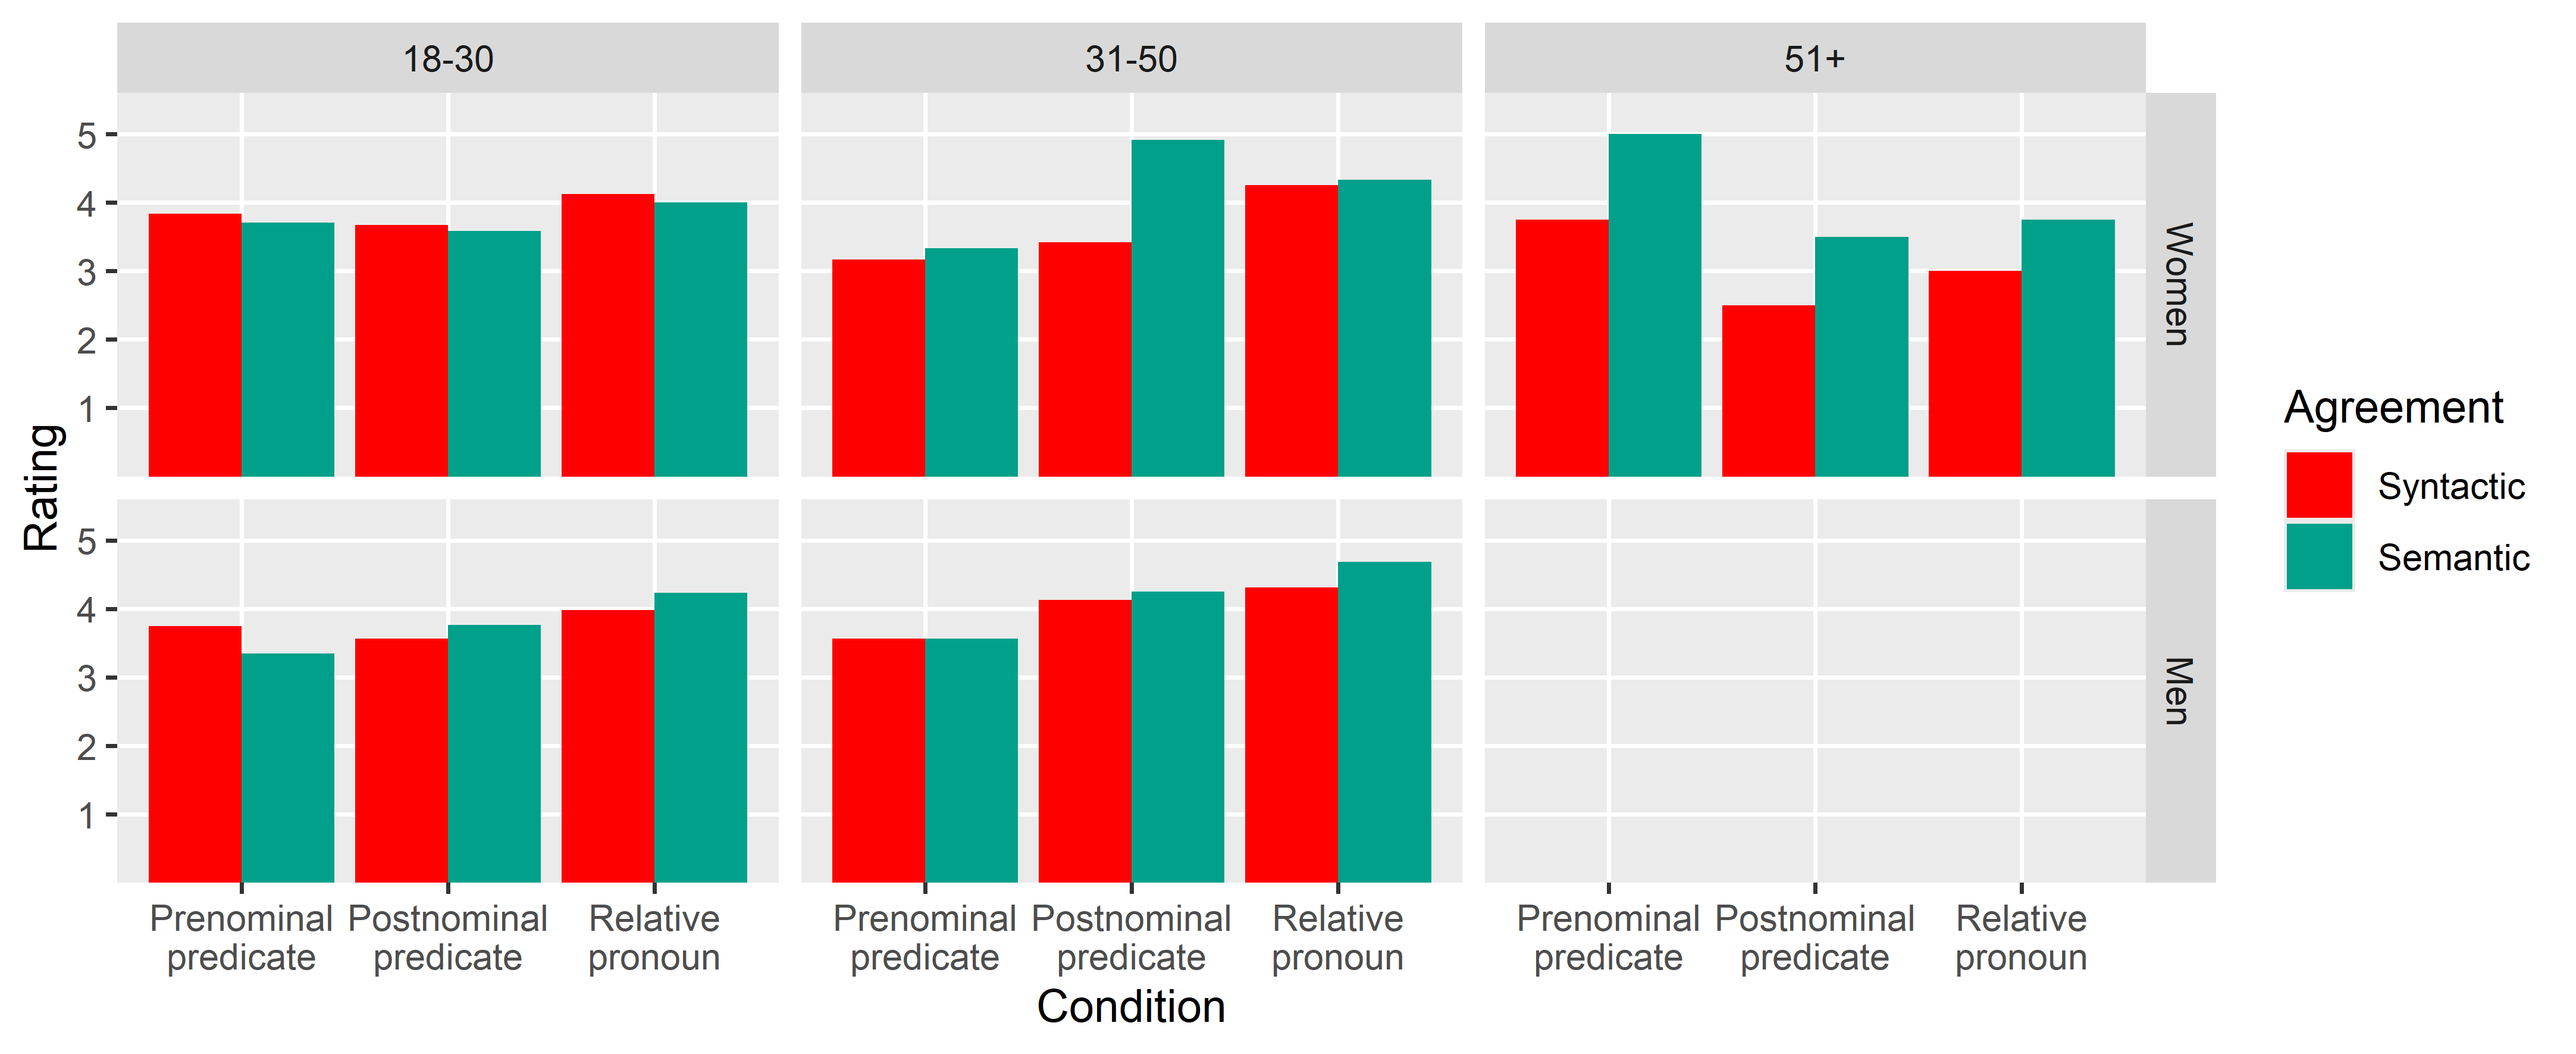
\includegraphics[scale=.7]{./images/expdemoprof.png}
  \caption{Average ratings of experimental items in Experiment 1 grouped by participants' age and gender.}
  \label{fig:prof-demo-plot}
\end{figure}

In the plot we can see that women in the youngest group have very similar ratings for all conditions with a slight preference towards syntactic agreement, while the middle group always prefers semantic agreement (it should be noted that the 51+ group here consists of only one person). For men, syntactic prenominal predicate agreement is either the same or better than semantic, while for other conditions they prefer semantic agreement. This is in line with Corbett's prediction that target before controller is more likely to be syntactic.

Results from this experiment were also anaylzed with a mixed-effects ordinal regression model, with agreement crossed with order and target type as predictors of acceptability rating and the same random effects as in the general model. The only significant effect in the model was the type of target: items with relative pronouns had significantly higher acceptability ratings than items with the predicates. However, the interaction between semantic agreement and the type of target was not significant. The list of coefficients from this model can be found in the Appendix (Table \ref{tab:coef-exp-prof}).

\subsection{Experiment 2}
In Experiment 2 the stimuli had depreciative forms. Table \ref{tab:exp-depr-summary} summarizes the results of this experiment.

% latex table generated in R 4.5.2 by xtable 1.8-8 package
% Sat May 30 20:32:22 2026
\begin{table}[h]
  \centering
  \begin{tblr}{
    hlines,vlines,
    cell{1}{1} = {r=2}{c},
    cell{1}{2} = {c=2}{c},
    cell{1}{4} = {c=2}{c},
    cell{1}{6} = {c=2}{c}
    }
    Agreement & Prenominal predicate & & Postnominal predicate & & Relative pronoun & \\
              & Mean & SD & Mean & SD & Mean & SD \\ 
    Semantic & 1.76 & 1.04 & 1.96 & 1.27 & 1.86 & 1.08 \\ 
    Syntactic & 1.59 & 0.94 & 1.55 & 0.95 & 1.70 & 1.03 \\ 
  \end{tblr}
  \caption{Means and standard deviations for acceptability ratings in all conditions in Experiment 1.}
  \label{tab:exp-depr-summary}
\end{table}

Ratings in Experiment 2 are visibily lower than in Experiment 1, but they never go below the average rating for ungrammatical controls. In all conditions, including prenominal predicates, semantic agreement is surprisingly rated higher than syntactic. Somewhat in line with the hypothesis about target-controller ordering, the preference for semantic agreement over syntactic grows when we move to postnominal predicate condition, where the controller is placed before the target. In contrast to the results from Experiment 1, there is no increase in acceptability of the items with relative pronouns.

Same as for Experiment 1, in Figure \ref{fig:depr-demo-plot} we can see the average ratings depending on the conditions, age group and gender of the participants.

\begin{figure}[h]
  \centering
  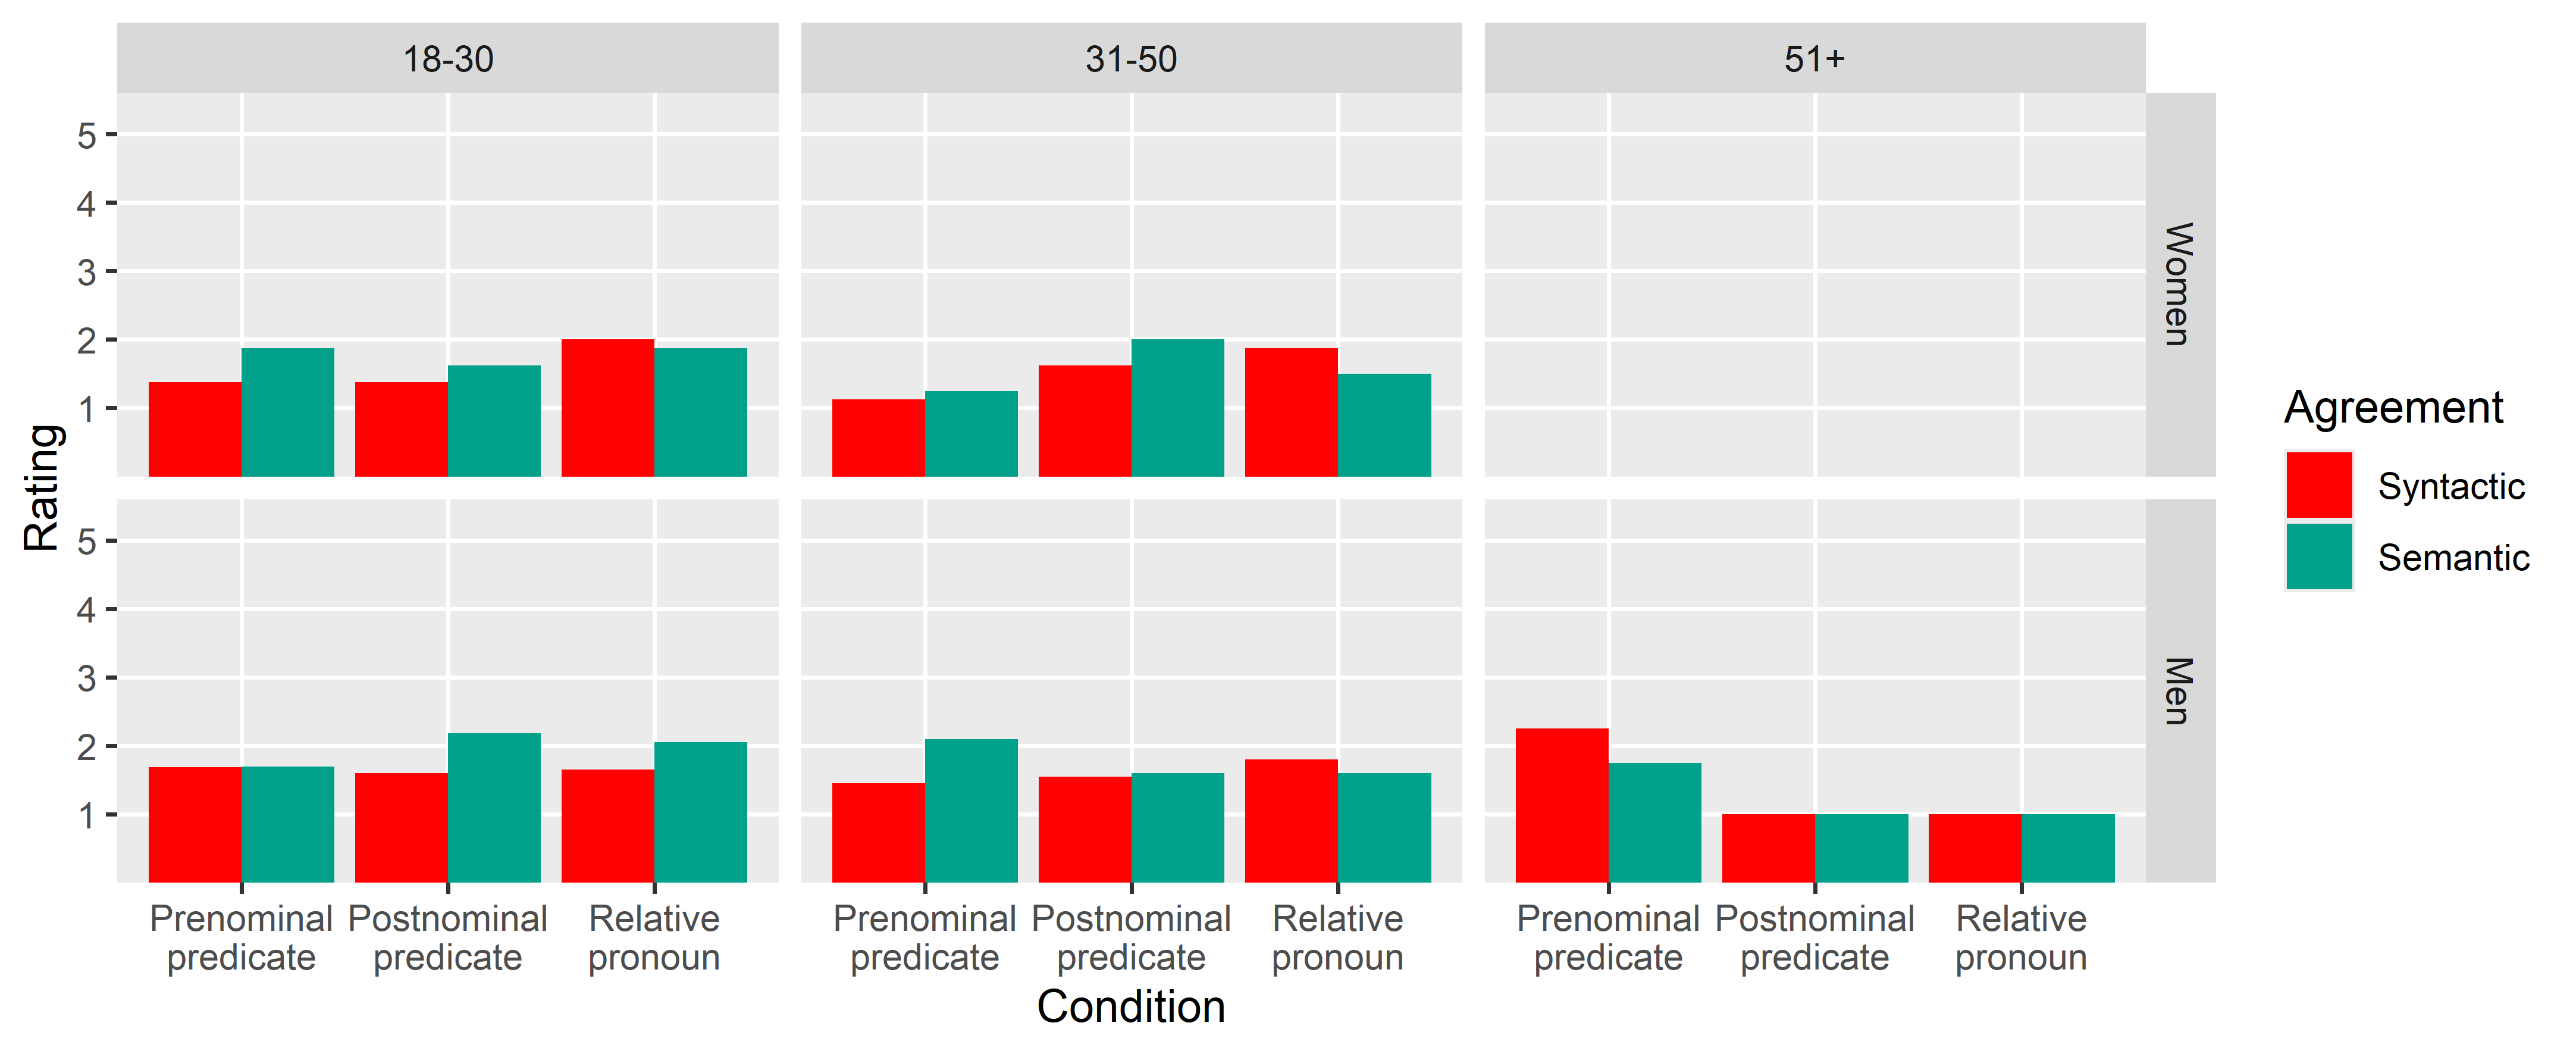
\includegraphics[scale=.8]{./images/expdemodepr.png}
  \caption{Average ratings of experimental items in Experiment 2 grouped by participants' age and gender.}
  \label{fig:depr-demo-plot}
\end{figure}

For relative pronouns women in both age groups there is a small preference for syntactic agreement, but for predicates semantic agreement is always rated higher. Men mostly prefer semantic agreement across age groups and conditions, with the exception of relative pronouns for men aged 31-50, where syntactic agreement is rated slightly higher (again, it should be noted that the oldest group consists of only one person here).

We analyzed the data from this experiment with the same mixed-effects ordinal regression model as in the previous section. There were the same fixed effects (agreement, order and target type) and the same random effects. In this model there were no significant effects, neither main effects nor interactions. The list of coefficients for this model is in the Appendix (Table \ref{tab:coef-exp-depr}).

\section{Discussion}
The only significant effect found in the model with all nouns was that items with depreciative forms were rated significantly lower than items with profession nouns. According to one of the hypotheses, semantic agreement with split hybrids is less acceptable than with lexical hybrids, but here the lower ratings for depreciative forms were independent of agreement: both items with semantic and syntactic agreement were rated as close to unacceptable if they used a depreciative form. There was no significant effect of interaction between agreement and type of noun.

Responses from two participants were filtered out because they rated all depreciative items as completely unacceptable. It seems that those participants thought the depreciative forms are unacceptable themselves and it is possible that this was the case to some extent with most of participants. Depreciative forms are a part of colloquial language and participants could feel that in the experimental settings those forms sound unnatural.

Based solely on descriptive statistics, in the results from Experiment 1 there seem to be some tendencies in the data in line with our hypotheses. On average semantic agreement is more acceptable with postnominal predicates than with prenominal predicates and target following the controller should make semantic agreement more acceptable, but the interaction between agreement and order was not significant. The items with relative pronouns have higher acceptability than items with predicates, and this difference was statistically significant but it was independent of agreement. Since the model showed no significant interaction between agreement and type of target, no conclusions can be drawn regarding acceptability of semantic agreement being higher for relative pronouns than for predicates, as was would be concurrent with the full constraint of the Agreement Hierarchy.

As for depreciative forms, semantic agreement had higher average ratings than syntactic agreement regardless of the condition. Semantic agreement is expected to be less acceptable in general with split hybrids, yet both in the corpus study and in the experimental study was surprisingly acceptable. It is possible that in the experiment, when participants were faced with sentences with ``incorrect'' forms of nouns, they preferred the version of the sentence with agreement that would be used with the ``correct'' form of noun. Even if there were some differences between acceptability in different conditions, none of them were statistically significant.

The interesting part of the interaction between the demographic profile of participants and the acceptability ratings in all conditions in Experiment 1 (with profession nouns) is the change in preferences between the youngest women and the group of women aged 31-50. In this experiment there were masculine nouns used for women and with recent efforts to use more feminitives to increase the visibility of women in male-dominated professions, younger women might be more inclined to prefer syntactic agreement with masculine nouns and use feminine agreement with feminine nouns, however uncommon these might be. In a study conducted by \cite{feminatywy2023}, where 300 university students (221 of whom were women) were asked to rate acceptability of feminitive forms, 58.4\% of all nouns had the average acceptability of at least 4 on a scale of 0 to 5 and 88.5\% were rated at least 3.

Another, slightly surprising, result is the differences between acceptability of semantic and syntactic agreement across conditions (Figure \ref{fig:exp-diffs}). Those differences are not significant according to any of the models, but for the sake of future directions it is worth discussing where those results can point. For prenominal predicate agreement the difference is similar for both experiments, but in opposite directions. The more interesting part are the differences in postnominal predicate and relative pronoun conditions. If we expect a monotonic change from syntactic attributive agreement to semantic pronoun agreement, we should see that for the middle points on that scale the difference between acceptability of semantic and syntactic agreement should be smaller than on the ends of the scale. Here, the difference is larger for postnominal predicate agreement and smaller for relative pronoun agreement. It would be beneficial for the future experimental studies to look into semantic and syntactic agreement with all targets on the Agreement Hierarchy.

As for other limitations of the current study, the ratings of items with depreciative forms could be affected by the colloquial nature of the forms themselves. These crucial in research the Agreement Hierarchy extended by generalized semantic agreement, because they are one of rare examples of split hybrids. If these are researched in the future however, it should be emphasised to participants that they should assume the experimental items appear in casual conversations. Another option would be to conduct a similar study, but with audio stimuli, so that participants hear the colloquial forms and are more likely to accept the informal context of the sentences.

The study had relatively little data, considering the number of experimental conditions in the design. Another future direction would be to conduct a similar study on a larger number of participants or with a larger number of items. With more participants there could also be more people in the oldest considered age group, which in the end consisted of only one person per experiment.

It would also be interesting to consider a different experimental design, for example a sentence recall task, where agreement chosen by participants when recalling the experimental items can show which agreement options they prefer. 
